\documentclass[12pt]{article}
\usepackage{geometry}
\usepackage{amsmath}
\usepackage{amsthm}
\usepackage{amssymb}
\usepackage{mathrsfs}
\usepackage{parskip}
\usepackage{enumerate}
\usepackage{stmaryrd}
\usepackage{listings}
\usepackage{float}
\usepackage[colorlinks]{hyperref}
\usepackage[x11names, rgb]{xcolor}
\usepackage[utf8]{inputenc}
\usepackage{tikz}
\usetikzlibrary{snakes,arrows,shapes}

\newtheorem{thm}{Theorem}[section]
\newcommand{\der}[1]{\ensuremath{\overset{#1}{\Rightarrow}}}
\numberwithin{equation}{subsection}

\begin{document}

\title{CS 360 Notes}
\author{Matthew Visser}
\date{Nov  3, 2011}
\maketitle

\section{Deterministic PDAs}

In a DPDA, every move is fixed.

\begin{itemize}
	\item If $ |\delta(q,a,X)| = 1$ for some letter $a$ then
		$|\delta(q,\varepsilon,X)|= 0$
	\item And $|\delta(q_0,a,X)|\le 1$ for all pairs $(q_0,a)$ (including $a =
		\varepsilon$) and $X$.
	\item For any state, letter, and stack symbol, we can only do one thing.
\end{itemize}

\subsection{Example}

Use the language
\begin{equation}
	L = \{ x \in \{a,b\}^* | n_a(x) > n_b(x) \}
	\label{eq:ex1}
\end{equation}

We have a DPDA starting at state ``equal''
\begin{figure}[H]
	
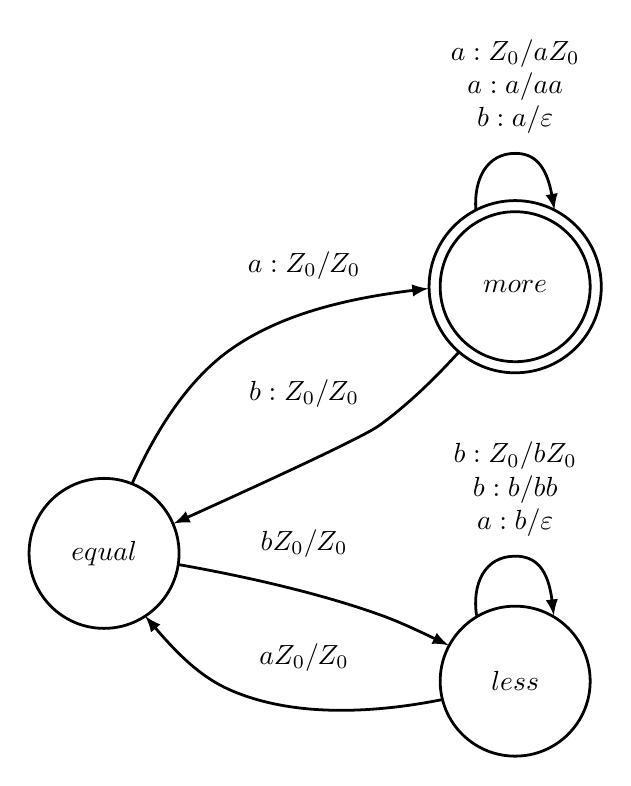
\begin{tikzpicture}[>=latex,line join=bevel,]
  \pgfsetlinewidth{1bp}
%%
\pgfsetcolor{black}
  % Edge: less -> equal
  \draw [->] (148.5bp,20.315bp) .. controls (127.12bp,16.065bp) and (96.269bp,13.175bp)  .. (72bp,24bp) .. controls (62.952bp,28.036bp) and (54.987bp,34.954bp)  .. (41.832bp,50.426bp);
  \definecolor{strokecol}{rgb}{0.0,0.0,0.0};
  \pgfsetstrokecolor{strokecol}
  \draw (99bp,35.5bp) node {$aZ_0/Z_0$};
  % Edge: less -> less
  \draw [->] (161.1bp,50.615bp) .. controls (159.38bp,61.973bp) and (164.02bp,72bp)  .. (175bp,72bp) .. controls (182.38bp,72bp) and (186.89bp,67.474bp)  .. (188.9bp,50.615bp);
  \draw (175bp,96bp) node {$ \begin{matrix} b:Z_0/bZ_0 \\ b:b/bb \\ a:b/\varepsilon \\ \end{matrix} $};
  % Edge: equal -> less
  \draw [->] (53.862bp,68.964bp) .. controls (73.906bp,65.416bp) and (102.18bp,59.485bp)  .. (126bp,51bp) .. controls (131.27bp,49.124bp) and (136.7bp,46.809bp)  .. (151.06bp,39.889bp);
  \draw (99bp,76.5bp) node {$bZ_0/Z_0$};
  % Edge: equal -> more
  \draw [->] (37.183bp,98.32bp) .. controls (44.282bp,114.36bp) and (55.68bp,134.22bp)  .. (72bp,146bp) .. controls (89.8bp,158.84bp) and (113.54bp,164.69bp)  .. (143.77bp,168.35bp);
  \draw (99bp,176.5bp) node {$a:Z_0/Z_0$};
  % Edge: more -> equal
  \draw [->] (154.78bp,145.53bp) .. controls (146.56bp,136.47bp) and (136.46bp,126.51bp)  .. (126bp,119bp) .. controls (120.25bp,114.88bp) and (87.387bp,99.701bp)  .. (52.027bp,83.723bp);
  \draw (99bp,130.5bp) node {$b:Z_0/Z_0$};
  % Edge: more -> more
  \draw [->] (160.84bp,196.62bp) .. controls (160.04bp,207.7bp) and (164.76bp,217bp)  .. (175bp,217bp) .. controls (181.88bp,217bp) and (186.27bp,212.8bp)  .. (189.16bp,196.62bp);
  \draw (175bp,241bp) node {$\begin{matrix} a:Z_0/aZ_0 \\ a:a/aa \\ b:a/\varepsilon \end{matrix}$};
  % Node: less
\begin{scope}
  \definecolor{strokecol}{rgb}{0.0,0.0,0.0};
  \pgfsetstrokecolor{strokecol}
  \draw (175bp,27bp) ellipse (27bp and 27bp);
  \draw (175bp,27bp) node {$less$};
\end{scope}
  % Node: equal
\begin{scope}
  \definecolor{strokecol}{rgb}{0.0,0.0,0.0};
  \pgfsetstrokecolor{strokecol}
  \draw (27bp,73bp) ellipse (27bp and 27bp);
  \draw (27bp,73bp) node {$equal$};
\end{scope}
  % Node: more
\begin{scope}
  \definecolor{strokecol}{rgb}{0.0,0.0,0.0};
  \pgfsetstrokecolor{strokecol}
  \draw (175bp,169bp) ellipse (27bp and 27bp);
  \draw (175bp,169bp) ellipse (31bp and 31bp);
  \draw (175bp,169bp) node {$more$};
\end{scope}
%
\end{tikzpicture}


	\caption{A DPDA describing the language in equation \ref{eq:ex1}}
	\label{fig:ex1}
\end{figure}

\subsection{Example}

A DPDA has no way of telling when its input is finished. Consider the language
of a palindrome.  Since we have no way of knowing how long our input is, we
can't accept these languages. If we accept too early, we reject the word, if we
accept that the end, we will still reject.

\subsection{Ambiguity and DPDA vs PDA}

A DPDA cannot accept an ambiguous grammar. If we convert from a DPDA to a NDPDA,
we will still have something that is unambiguous.

\begin{tabular}{p{0.5\textwidth}|p{0.5\textwidth}}
	\multicolumn{1}{c|}{PDA} & \multicolumn{1}{c}{DPDA} \\
	\hline
	\begin{itemize}
		\item Also an NFA
		\item accepts context-free languages
	\end{itemize}
	&
	\begin{itemize}
		\item A DFA
		\item Accepts context-free languages
		\item The context-free languages that are accepted are unambiguous.
	\end{itemize}
\end{tabular}

\section{Chomsky Normal Form}

\begin{itemize}
	\item $A \to BC$ where $A,B,C$ are variables.
	\item $A \to a$ where $A$ is variable and $a$ is terminal
\end{itemize}

\begin{thm}
	Given any CFG $G$, there exists a CFG $G'$ in LNF that accepts the same
	language as $G$ except for $\varepsilon$.
\end{thm}

A variable $A$ is \emph{nullable} If $A \der{*} \varepsilon$

If $A$ is nullable, and there is a rule $B \to AC$, we could replace it
with $B \to C$

Base: $A \to \varepsilon$

Recursive case:  $A \to B_1B_2\dots B_k$ where $B_1$ is nullable
$\forall 1\le i \le k$.

\begin{itemize}
	\item $(A,B)$ is a \emph{unit pair} if $A \der B$.
	\item $(A,A)$ is a unit pair for any variable $A$.
	\item If $(A,B)$ is a unit pair and $B \to C$ then $(A,C)$ is a unit pair.
\end{itemize}

Suppose we have a grammar in CNF with $n$ variables. Consider a parse tree in
that grammar for the word $z,\ |z|=k$.


\end{document}
% vim: tw=80
